\documentclass[a4paper,11pt]{article}
\usepackage[utf8]{inputenc}
\usepackage[english]{babel}
\usepackage{authblk}
\usepackage{graphicx}
\usepackage{mathptmx}
\usepackage[singlespacing]{setspace}
\usepackage[margin=1in,top=0pt]{geometry}
\usepackage{fancyhdr}
\usepackage{multicol}


\renewcommand{\headrulewidth}{0pt}
\pagestyle{fancy}

\graphicspath{{images/}}

\title{\vspace{-1ex}Aviation Accident Report Clustering\vspace{-1ex}}

\author[]{John Bollenbacher
} 

\affil{Observatory on Social Media\\
Indiana University, Indiana, USA
}
 
\date{}

\begin{document}

\maketitle
\thispagestyle{fancy}

\vspace{-8ex}

\begin{figure}[h!]
  \centering
  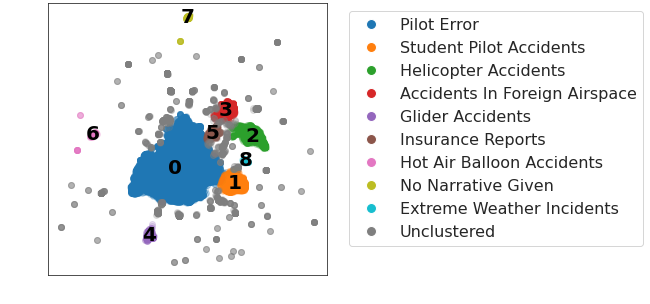
\includegraphics[width=0.9\textwidth]{cluster_plot.png}
  \label{fig:clusters}
  \vspace{-4ex}
  \caption{Topic clusters from aviation accident reports, presented in order of most to least common.}
\end{figure}


\begin{multicols}{2}

\section{Intro}

The Federal Aviation Administration (FAA) meticulously collects data on aviation accidents in order to improve and maintain flight safety. In this brief exercise, we examine a collection of FAA accident reports and attempt to group the accidents into categories that might help us better understand the aviation accidents. 

\section{Methods}
Our first step in working with text data is always to manually inspect the data for regularities. In this case, we find that the first sentence of each report is a boilerplate evidentiary statement telling us how the information was collected, which we safely can remove for this exercise.  We also standardize common acronyms and abbreviations in order for our machine learning models to be better able to understand the text data. 

Next, we need to turn our text data into numerical vectors so we can work with it more easily.  To do this, we can use the deep learning language model called BERT, which can take in a short body of text and produce a vector which represents it; these "embedding vectors" are defined so that texts which are similar to each other have vectors which are close together in the embedding space. 

Finally, we want to visualize and cluster these vectors, so we can identify meaningful groups of content and better understand what kinds of aviation crash reports we have in our data set. To do this, we'll plot our data in 2D, and use a clustering method called HDBSCAN to identify the clusters in the data (See Figure 1). After we've identified our clusters, we again manually inspect the text data to figure out what each cluster is about. 

\section{Results}

We find that the most common category of accident in our data is reports describing incidents of pilot error.  We also find a number of other causes, such as student pilot mistakes and extreme weather events.  

However, not all the clusters are so useful.  Our methods identified a number of clusters that are only about the type of aircraft, for instance helicopters, gliders, and hot air balloons. We also identified a number of clusters that are primarily about the sort of language used, rather than the incident itself; for instance there's a cluster which contains foreign location names ("Accidents in Foreign Airspace") and a cluster which seems to describe primarily information of interest to insurers ("Insurance Reports"), such as injuries, ownership of the aircraft, and pilot liabilities. 

Finally, we have a number of data points which did not fall into any cluster ("Unclustered"), and another small set of data points which did not have any text description at all ("No Narratives Given"). 

\vspace{-3ex}



\end{multicols}


\end{document}
